\chapter {Description formelle de l'éditeur de composants métiers caractéristiques}

\subsection{Présentation de l'éditeur}
L'embryon de plateforme existant pour la méthode FORM/BCS a été développé en Java en utilisant le framework Eclipse EMF(Eclipse Modeling Framework). EMF est un environnement de modélisation et de génération de code qui facilite la construction d'outils et d'applications sur les modèles de données structurées Il est basé sur l'Ingenierie Dirigée par les Modèles (IDM),; l'approche de développement IDM consiste à séparer les spécification fonctionnelles d'un système d'un système de son implémentation Elle préconise pour ce faire de construire quatres principaux modèles pour aboutir à la génération du code source 
\begin{itemize}
	\item CIM (Computational Independent Model) qui modélise les exigences fonctionnelles du système
	\item PIM (Platform Independent Model) ou encore modèle conceptuel qui est un modèle abstrait, indépendant de toute plateforme d'exécution 
	\item PSM (Platform Specific Model) qui est un modèle contenant les détails propres à une plateforme donnée
	\item PDM (Platform Dependent Model) c'est un modèle qui intègre les spécificités d'une plateforme. Il naît du couplage entre le PIM et une PSM donnée.
	\item Le code source est généré à partir de la PDM. 
	\end{itemize}
	
	Concrètement, EMF génère du code source en transformant différents modèles et génère des éditeurs textuels ou graphique. Le point d'entrée est un modèle appelé Ecore, c'est le Méta-modèle d'EMF et est indépendant de la plateforme d'execution car ne contient aucne information à propos des packages ou des classes Java. Ce dernier peut être spécifié en utilisant l'éditeur graphique qu'offre EMF ou en important des interfaces Java, un diagramme de classe UML ou un schéma XML. Le méta-modèle Ecore étant indépendant de toute plateforme d'exécution, pour générer du code Java, il faut spécifier un modèle de génération qui contient les informations de plateforme (packages, classes...): c'est le \textsl{genmodel}; Eclipse permet de le générer automatiquement à partir du modèle Ecore. Le plugin EMFTEXT permet de générer des éditeurs pour les DSL (Domain Specific Language) avce des fonctionnalités avancées telles que l'autocomplétion, la coloration du texte, la personnalisationde la syntaxe, le rapport instantané des erreurs etc. C'est ce plugin qui a été utilisé pour la réalisation de l'embryon de plateforme pour le projet REAL. 

\begin{figure}[h!]
  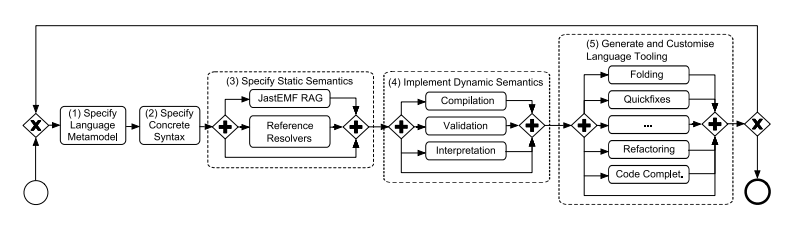
\includegraphics[scale=0.7]{images/EMFTEXT_process.png}
  \caption{Processus de développement d'un langage avec EMFTEXT}
  \label{fig:EMFTEXT_process}
\end{figure}

La génération d'un éditeur sophistiqué pour un nouveau langage necessite juste quelques étapes de spécification et de génération avec EMFTEXT comme le montre la figure \ref{fig:EMFTEXT_process}. Ces étapes sont alors les suivantes:
\begin{enumerate}
	\item spécifier du métamodèle Ecore
	\item spécifier de la syntaxe concrète en utilisant CS
	\item (optionnelle) spécifier la sémantique statique 
	\item (optionnelle) implémenter la sémantique dynamique 
	\item générer et (optionellement) modifier l'éditeur, par exemple en adaptant la complétion de code, la mise en valeur de la syntaxe etc.
\end{enumerate}

De ces étapes, seules les étapes (1) et (2) sont obligatoires ainsi que la génération du code de l'éditeur (étape 5). C'est par ces dernières que plugin REAL a été généré. 
\subsection{Description formelle}

